% -----------------------------------------------------------------------------
\section{(Proposal A)\\Predictive control for transitioning WWTPs\\ into self-sufficient WRRFs} \sectioncover
% -----------------------------------------------------------------------------
\begin{frame}[c]
\frametitle{Predictive control, operating WWTPs as self-sufficient WRRFs} \justifying

\vskip1em

\boxHighlight[0.9\textwidth]{ \centering
    We consider the task of operating a \textbf{biological wastewater treatment plant} (WWTP, secondary treatment) as a \textbf{water resource recovery facility} (WRRF)
}

\vfill

\begin{center}
    \includegraphics<1>[width=\textwidth]{figs/ControlFramework_01}%
    \includegraphics<2>[width=\textwidth]{figs/ControlFramework_02}%
\end{center}

\vfill

\end{frame}

%------------------------------------------------------- 
\begin{frame}[t]
\frametitle{Predictive control, general architecture and specific configuration}\justifying

\vskip0.66em

\begin{columns}
	\column[t]{0.5\textwidth}
	\begin{center}
		\vskip-1.5em
		\includegraphics<1>[width=0.98\columnwidth]{figs/Control_Diagram_Isolated}% 
		\includegraphics<2>[width=0.98\columnwidth]{figs/Control_Diagram_Isolated_H1}% 
		\includegraphics<3>[width=0.98\columnwidth]{figs/Control_Diagram_Isolated_H3}% 
		\includegraphics<4>[width=0.98\columnwidth]{figs/Control_Diagram_Isolated_H2}% 
	\end{center}

	\column[t]{0.49\textwidth}
	We design a \textbf{model-based} output-feedback controller
    \begin{equation*}
        \Sigma \coloneqq \left\{
            \begin{aligned}
                \textstyle\frac{d}{dt}\clX{x(t)} &= f(\clX{x(t)}, \clW{w(t)}, \clU{u(t)})   & \text{\footnotesize\color{gray}(dynamics)} \\
                \clY{y(t)}   				     &= g(\clX{x(t)}, \clW{w(t)}, \clU{u(t)})   & \text{\footnotesize\color{gray}(measurements)} \\
                \clY{z(t)}   				     &= h(\clX{x(t)}, \clW{w(t)}, \clU{u(t)})   & \text{\footnotesize\color{gray}(performance)}
            \end{aligned}
        \right.
    \end{equation*}

	\vskip0.5em
	which autonomously operates the plant in cycles	
	\begin{center}
		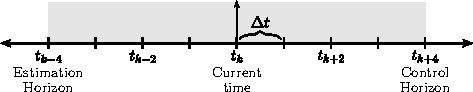
\includegraphics[width=0.9\columnwidth]{figs/Control_Diagram_Time}
	\end{center}
\end{columns}

\vskip2em

\only<2>{\centering%
    \begin{tcolorbox}[colframe=monokaiBG!33!white, colback=white, width=\textwidth, rounded corners]
    \vspace*{-1.66em}
    \begin{tcolorbox}[frame empty, boxsep=-5pt, colback=white, width=19em]
        \textsc{Operating point optimizer} | $\mathrm{OPO}(\cdot)$
    \end{tcolorbox} 
    \vspace*{-0.33em}
    \begin{columns}
    \column[c]{0.45\columnwidth}
    \vskip-2em
    \begin{align*}
        \underset{x_k,~ u_k}{\text{minimize}} \quad
        & \left\| 
                \clP{\begin{bmatrix} W_{z|\text{ref}} & \\ & W_{u|\text{ref}} \end{bmatrix} }
                \begin{bmatrix} 
                    \clY{z_k - \bar{z}^{\text{ref}}_k} \\ 
                    \clU{u_k - \bar{u}^{\text{ref}}_k} 
                \end{bmatrix} 
        \right\|_2^2 \\
        \underset{}{\text{subject to}} \quad
            &  0  = f(\clX{x_k}, \clW{\bar{w}^{\text{ref}}_k}, \clU{u_k}) \\[-2ex]
            % & z_k = h(x_k, \bar{w}^{\text{ref}}_k, u_k) \label{eq: WRRF_OPO_c}\\
            & \clY{z_k \in \mathcal{Z}_{\text{ref}}}, ~~ \clX{x_k \in \mathcal{X}_{\text{ref}}}, ~~ \clU{u_k \in \mathcal{U}_{\text{ref}}}
    \end{align*}

    \column[c]{0.1em}\rule{0.5pt}{6em}

    \column[c]{0.54\columnwidth} 
    \vskip-2em
    \begin{equation*}
        \hspace*{-1em}
        \Sigma^{\delta|k} \coloneqq \left\{
        \begin{aligned}
            \clP{z}\clX{x^{\delta}[n]} &= \clP{A_k} \clX{x^{\delta}[n]} + \clP{B_{w|k}} \clW{w^{\delta}[n]} + \clP{B_{u|k}} \clU{u^{\delta}[n]} \\
                           \clY{y^{\delta}[n]} &= \clP{C_k} \clX{x^{\delta}[n]} + \clP{D_{w|k}} \clW{w^{\delta}[n]}
        \end{aligned}
        \right.
    \end{equation*}
    \end{columns}
    \end{tcolorbox}
}%
\only<3>{\centering%
    \begin{tcolorbox}[colframe=monokaiBG!33!white, colback=white, width=\textwidth, rounded corners]
        \vspace*{-1.66em}
        \begin{tcolorbox}[frame empty, boxsep=-5pt, colback=white, width=20.5em]
            \textsc{Model predictive controller} | $\mathrm{MPC}(\cdot)$
        \end{tcolorbox} 
        \vspace*{-2em}
        \begin{align*}
            \underset{\clU{u^{\delta}[\cdot]},~ \clX{x^{\delta}[\cdot]}}{\text{minimize}} \quad
            & \sum_{n=0}^{N_c-1} \left\| 
                    \clP{\begin{bmatrix} W_{x|n} & \\ & W_{u|n} \end{bmatrix}} 
                    \begin{bmatrix} 
                        \clX{x^{\delta}[n]}  \\ 
                        \clU{u^{\delta}[n]}
                    \end{bmatrix} 
            \right\|_2^2 + \left\| \clP{W_{x|N_c}} \clX{x^{\delta}[N_c]} \right\|_2^2 \\
            \underset{}{\text{subject to}} \quad
                &  \Sigma^{\delta|k} \text{ with } \clW{w^{\delta}[n] = \hat{w}^{\delta}_{N_e{-}1}} \text{ and } \clX{x^{\delta}[0] = \hat{x}^{\delta}_{N_e}} \\[-1.5ex]
                &  \clX{x^{\delta}_{\text{lb}} \preceq x^{\delta}[n] \preceq x^{\delta}_{\text{ub}}}, 
                ~~ \clU{u^{\delta}_{\text{lb}} \preceq u^{\delta}[n] \preceq u^{\delta}_{\text{ub}}}
        \end{align*}
    \end{tcolorbox}
}%
\only<4>{\centering
    \begin{tcolorbox}[colframe=monokaiBG!33!white, colback=white, width=\textwidth, rounded corners]
        \vspace*{-1.66em}
        \begin{tcolorbox}[frame empty, boxsep=-5pt, colback=white, width=19em]
            \textsc{Moving horizon estimator} | $\mathrm{MHE}(\cdot)$
        \end{tcolorbox} 
        \vspace*{-2em}
        \begin{align*}
            \underset{\clW{w^{\delta}[\cdot]},~ \clX{x^{\delta}[\cdot]}}{\text{minimize}} ~~
            & \sum_{n=0}^{N_e-1} \left\| 
                    \clP{\begin{bmatrix} W_{y|n} \hspace*{2.6em} \\ \hspace*{2.6em} W_{w|n} \end{bmatrix}} \hspace*{-0.25em}
                    \begin{bmatrix} 
                        \clY{y^{\delta}[n] {-} y^{\text{data}|\delta}_n}  \\ 
                        \clW{w^{\delta}[n] {-} w^{\text{data}|\delta}_n}  
                    \end{bmatrix} 
            \right\|_2^2 {+} \left\| \clP{W_{y|N_e}} \clY{\big( y^{\delta}[N_e] {-} y^{\text{data}|\delta}_{N_e} \big)} \right\|_2^2 \\
            \underset{}{\text{subject to}} ~~
                &~ \Sigma^{\delta|k} \text{ with } \clU{u^{\delta}[n] = u^{\text{data}|\delta}_n}\\[-1.5ex]
                &~ \clX{x^{\delta}_{\text{lb}} \preceq x^{\delta}[n] \preceq x^{\delta}_{\text{ub}}}, 
                ~~ \clW{w^{\delta}_{\text{lb}} \preceq w^{\delta}[n] \preceq w^{\delta}_{\text{ub}}}. 
        \end{align*}
    \end{tcolorbox}
}%

\end{frame}

% -----------------------------------------------------------------------------
\begin{frame}[t]
\frametitle{Predictive control, experimental study}\justifying
	
\vskip1em

\boxHighlight[0.9\textwidth]{ \centering
    We consider the task of operating a \textbf{biological wastewater treatment plant} (WWTP, secondary treatment) as a \textbf{water resource recovery facility} (WRRF)
}

\vfill

\begin{columns}
	\column[c]{0.45\textwidth}%
	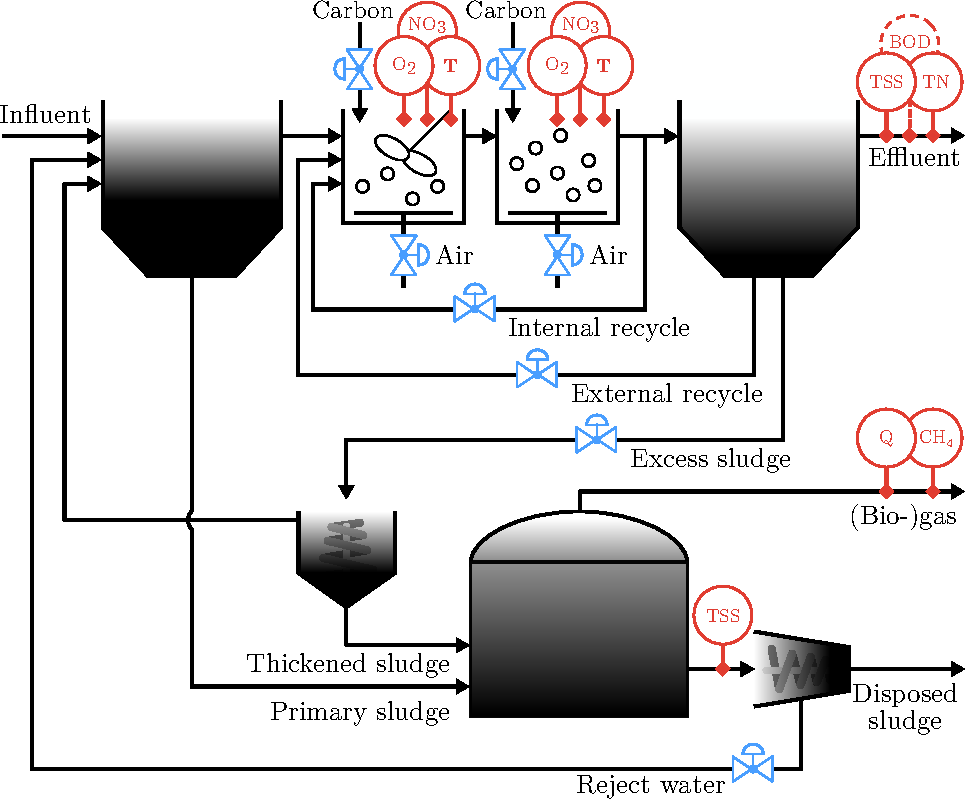
\includegraphics[width=\columnwidth]{figs/WRRF_Schematic_Instrumented_Colors}

	\column[c]{0.54\textwidth}
	\begin{itemize}
		\item {\color{monokaiOrange}\sc Primary objective:}\\
		on demand, produce effluent water of specific quality
		\vskip0.5em
		\begin{center}
            \begin{tabular}{@{}c ccc@{}} \toprule
                Water class & \multicolumn{3}{c}{Biochemical profile}                   \\\midrule
                            & {\small TSS}      &    {\small BOD}   &    {\small  TN}   \\\cmidrule{2-4}
                \textbf{A}  & $\leq 30$ g/m$^3$ & $\leq 10$ g/m$^3$ & $\leq 15$ g/m$^3$ \\
                \textbf{B}  & $\leq 30$ g/m$^3$ & $\leq 15$ g/m$^3$ & $\leq 30$ g/m$^3$ \\
                \textbf{C}  & $\leq 30$ g/m$^3$ & $\leq 20$ g/m$^3$ & $\leq 45$ g/m$^3$ \\\bottomrule
            \end{tabular}
		\end{center}
		\vskip1.5em
		%
		\item {\color{monokaiOrange}\sc Secondary objective:}\\
		produce biogas to ensure nonpositive energy cost index,
		\begin{multline*}
			\text{ECI} = \text{AE} + \text{PE} + \text{ME} - \eta_{E} \text{MP} \\
                            + \max(0, \text{HE} - \eta_{H}\text{MP})
		\end{multline*}
	\end{itemize}
\end{columns}

\vfill

\end{frame}

%------------------------------------------------------- 
\begin{frame}[c]
\frametitle{Predictive control, experimental study (cont.)}\justifying

\vfill

\begin{center}
	\only<1>{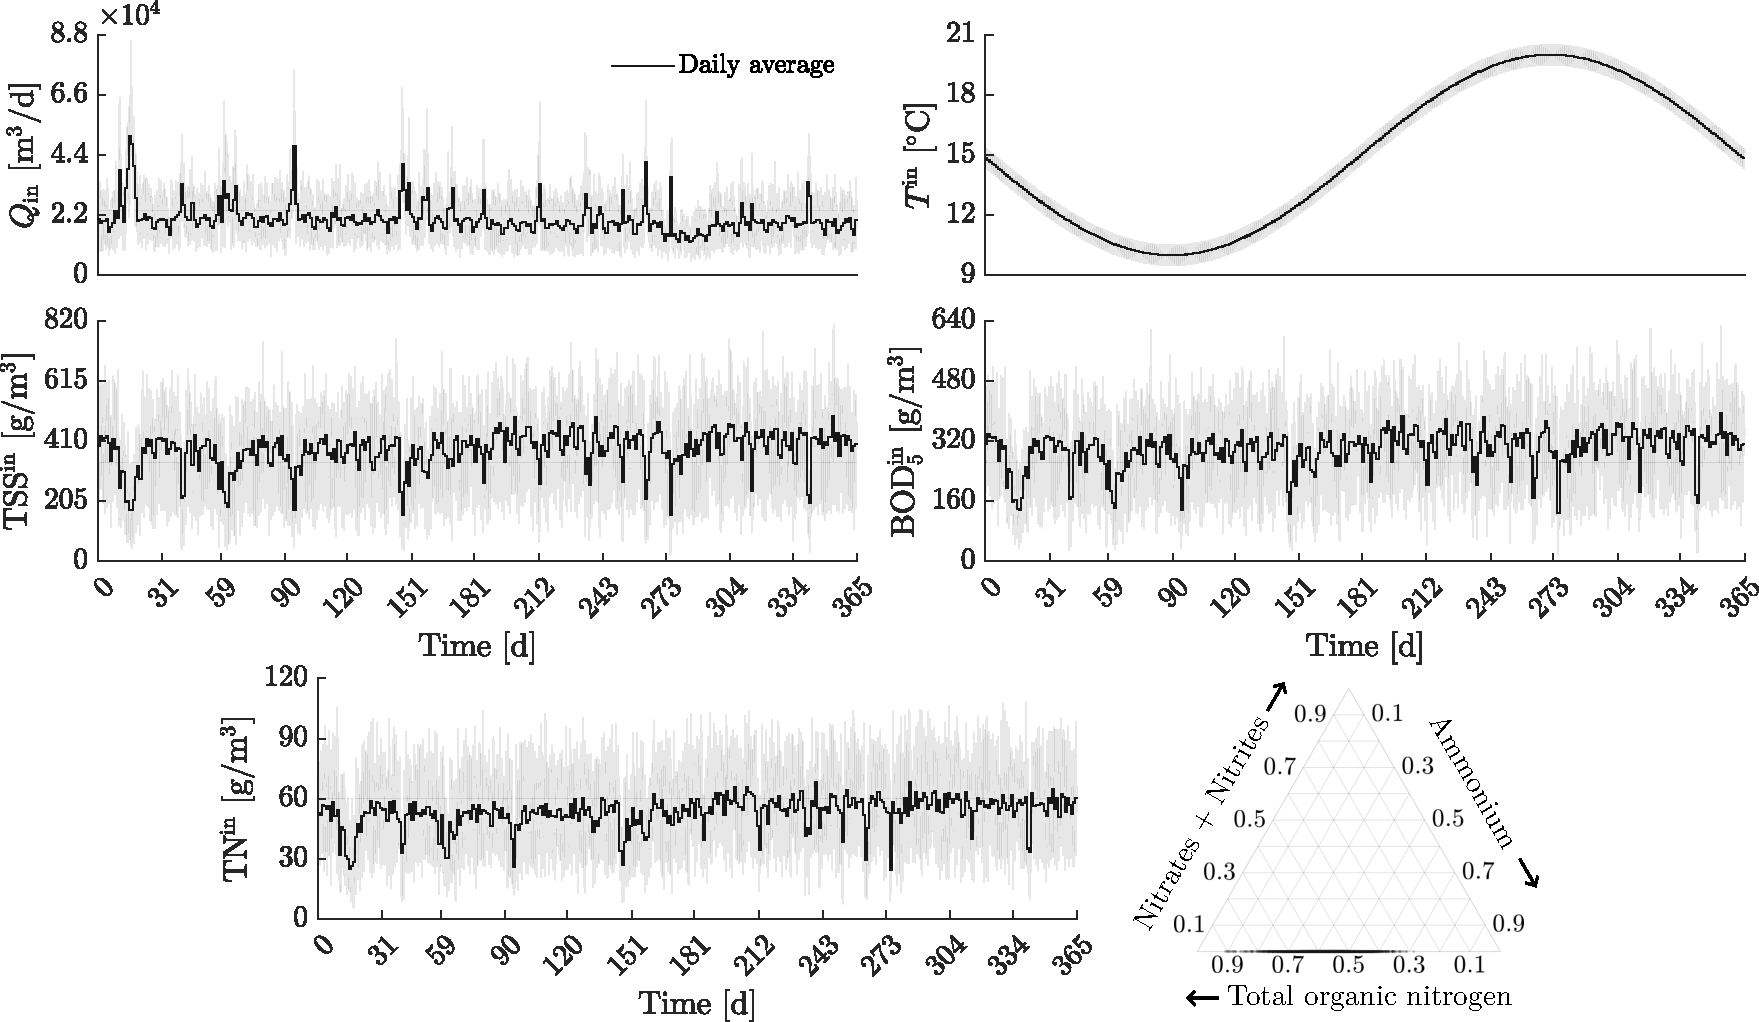
\includegraphics[width=0.9\textwidth]{figs/Simulation_Influent}}%
	\only<2>{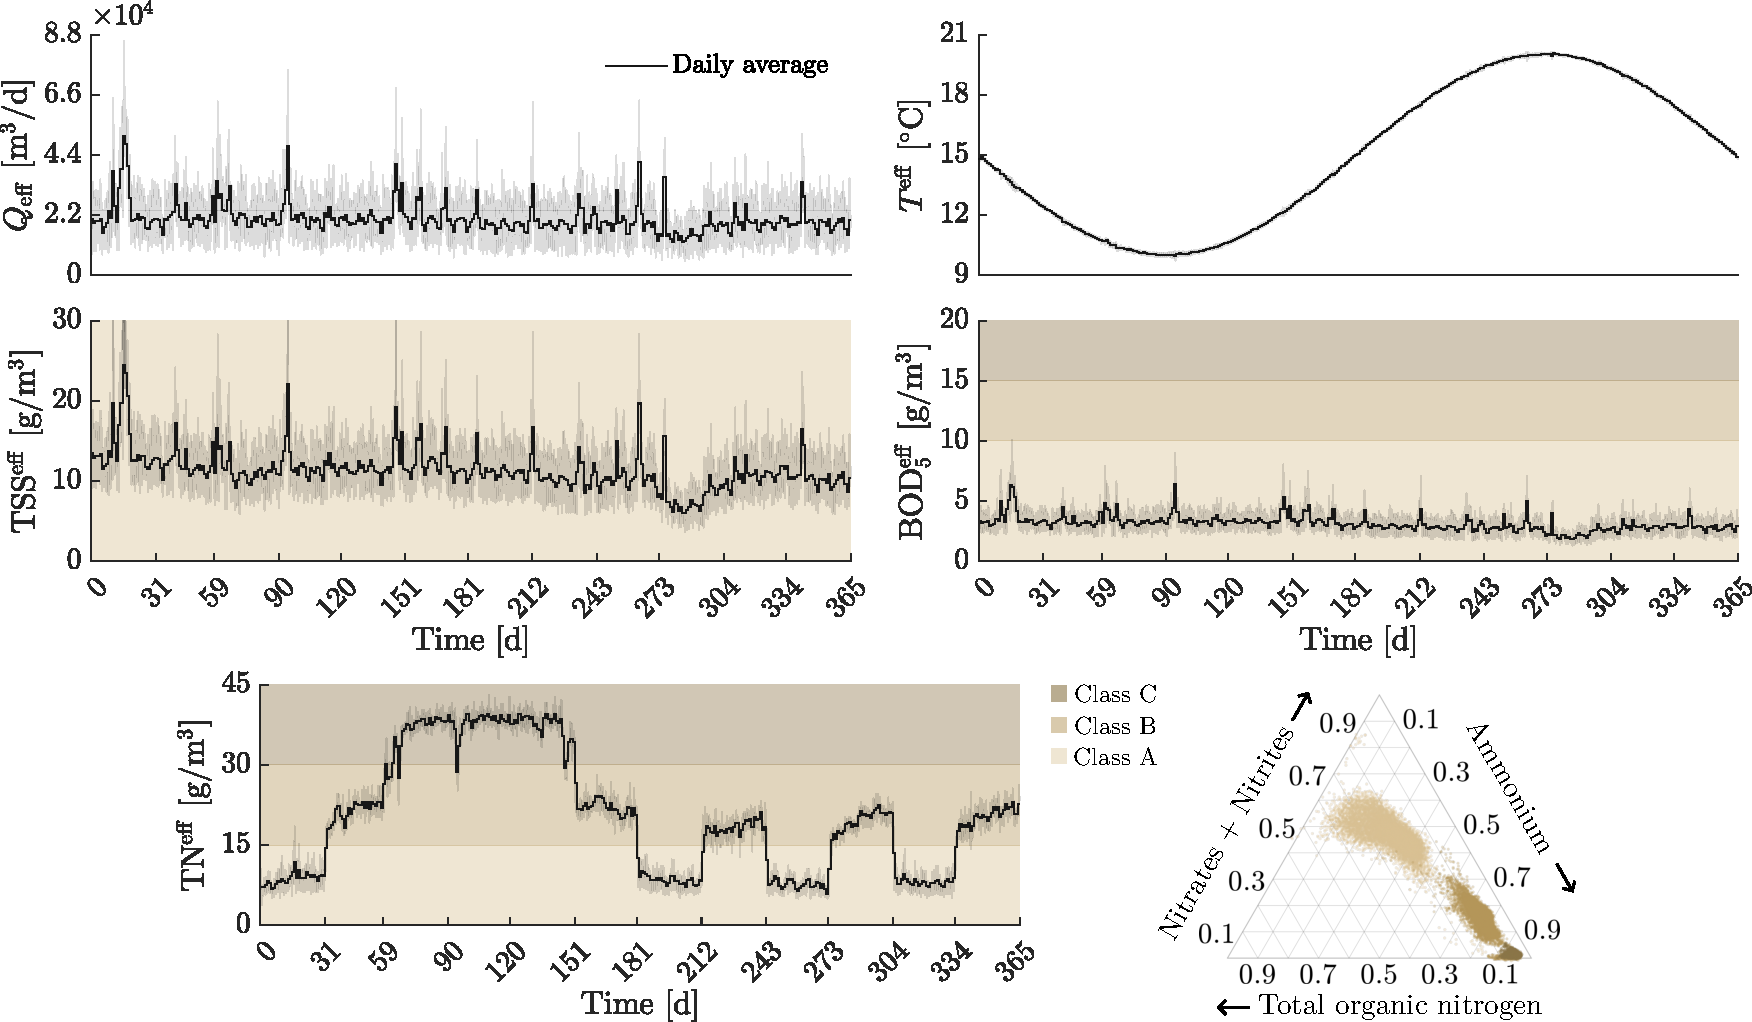
\includegraphics[width=0.9\textwidth]{figs/Simulation_Effluent}}%
	\only<3>{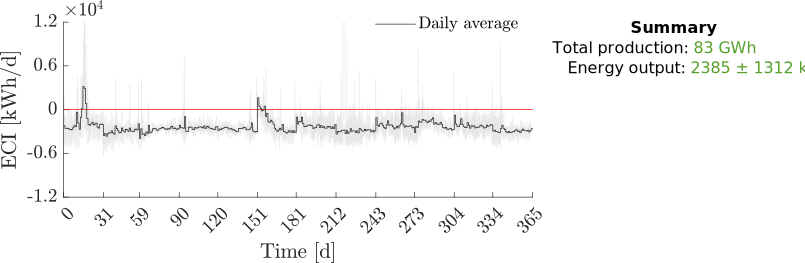
\includegraphics[width=0.8\textwidth]{figs/Simulation_ECI}}%
\end{center}

\vfill

\only<3>{
\boxInfo[0.85\textwidth]{ \centering
    The controller renders the WRRF energetically self-sufficient (on average)
}
}

\end{frame}
%------------------------------------------------------- 
